\subsection{Let the world know that you exist}

No matter how optimized the representation of the data is and how available we make it, if users are not aware
of the existence of the resource, they can not use it.

\subsubsection*{Suggested strategies} 

% TODO: need more
The best way is to advertise the product in the right media with right format.

\subsubsection*{In the context of Aire Guru \ldots}

Our website is implemented for the city of Málaga, so we are currently working to publicize it in this city.
It is currently available in the open data portal in the web site tab (https://datosabiertos.malaga.eu/aplicaciones). \\

Aire Guru participated in the first open data reuse contest organized by the Málaga City Council (http://cemi.malaga.eu/es/novedades/detalle/1-Concurso-de-Reutilizacion-de-Datos-Abiertos-del-Ayuntamiento-de-Malaga)
and was a finalist in the web page category. This provided valuable exposure.

\begin{figure}[ht]
    \centering
    \subfigure[Advertising in the open data portal of Málaga]
        {\centering 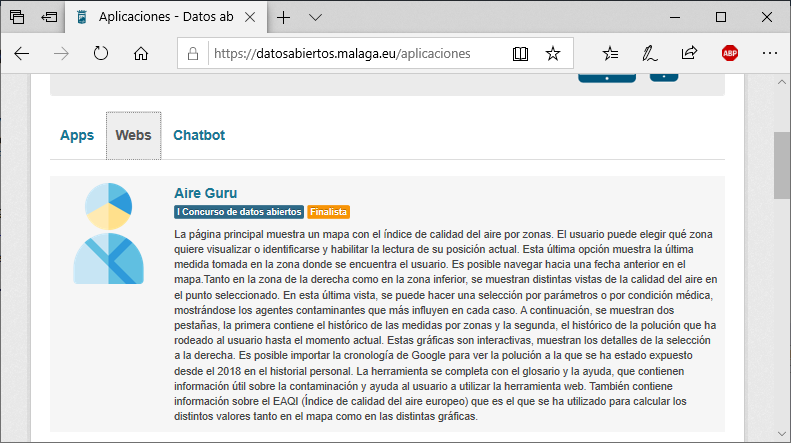
\includegraphics[width=6cm]{Figure_4_5_1_a_aireGuruAdvertised}}
    \hfill
    \subfigure[Finalist]
        {\centering 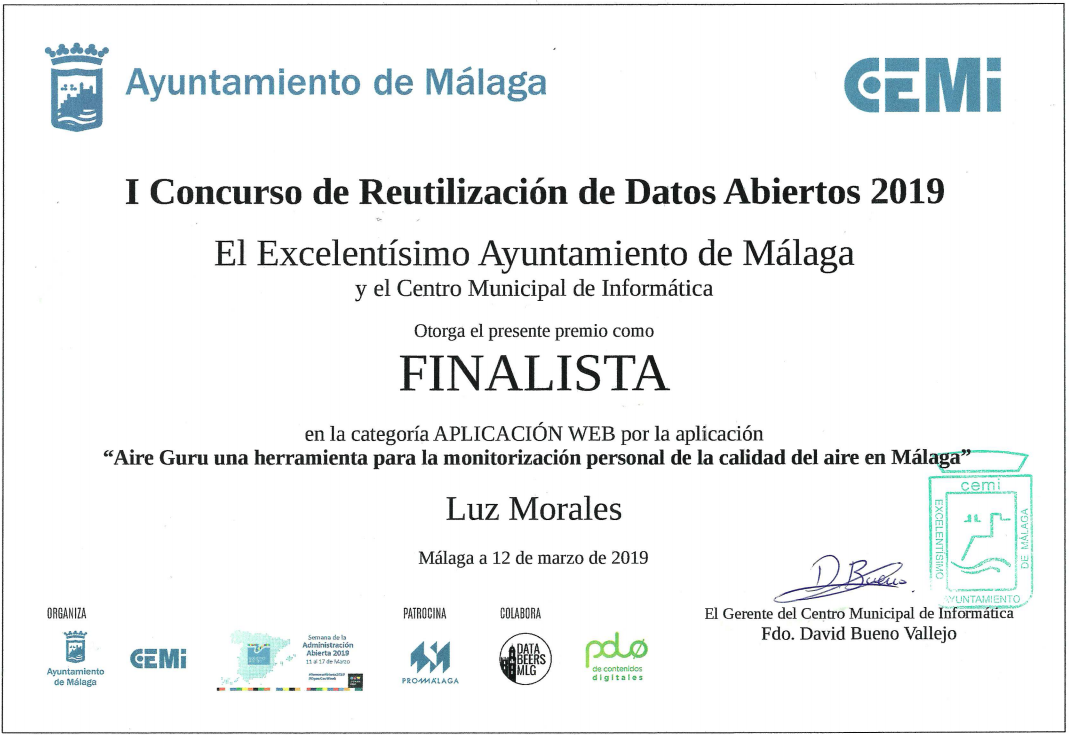
\includegraphics[width=5cm]{Figure_4_5_1_b_aireGuruFinalistCertificate}}
    \caption{I Contest of reuse of open data. Málaga's town hall}
\end{figure}

\begin{center}
    \bf{ (a) Advertising in the open data portal of Málaga     (b) Finalist   \\
    Figure 4.5.1. I Contest of reuse of open data. Málaga's town hall}
\end{center}